\section{System model}

\subsection{Model-View-Controller}


\begin{figure}[h]
	\centering
	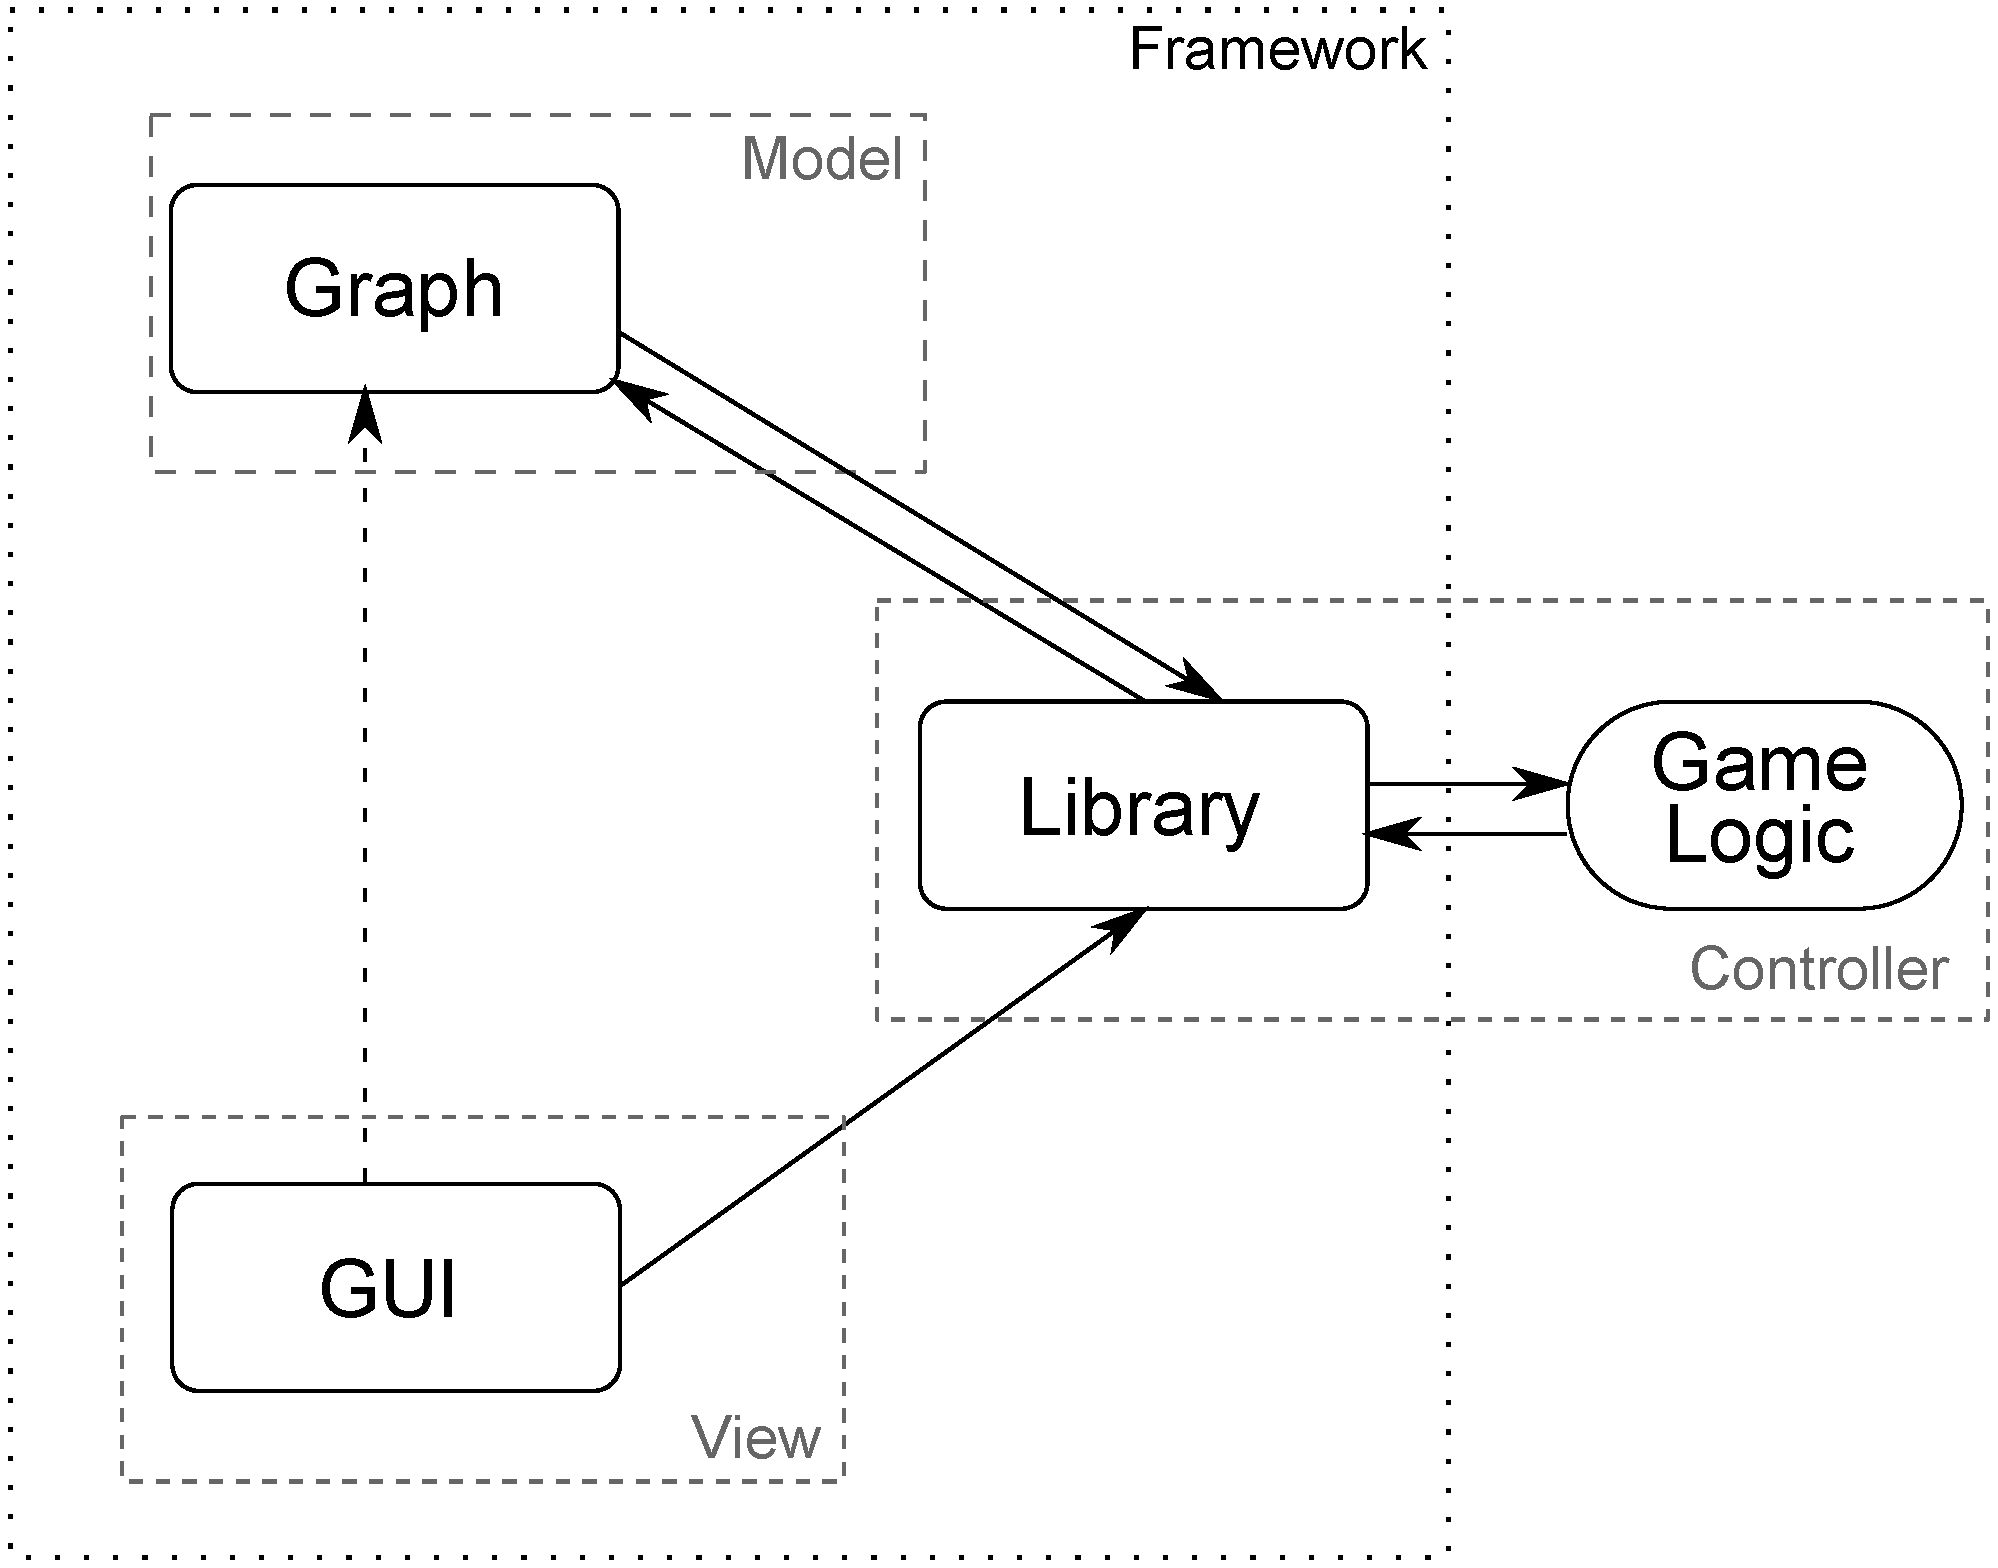
\includegraphics[width=0.8\textwidth]{mvc.pdf}
	\caption{Diagram showing the realization of the \gls{MVC} design pattern by the framework.}
	\label{img:MVC}
\end{figure}

\begin{description}
	\item[Model] The model contains the structure of the \gls{game}['s] current \gls{graph}.
	\item[GUI] The \gls{gui} is responsible for displaying the game, including the \gls{graph} represented by the model and the menu (see Section \ref{REF:GUI_GAME}). It listenes to changes of the model. It also receives user input (e.g. mouse clicks) and passes them to the controller.
	\item[Library] The library acts as an interface between the game and the remaining parts of the framework. It preprocesses the user input and notifies the game logic, by calling it's respective event listener. Furthermore it provides methods, which can be called by the game logic, that are used to access and modify the \gls{graph} stored in the model.
	\item[Game Logic] The Game Logic is the component created by the \gls{developer}. It decides how the user input is handled and what modifications have to be applied to the \gls{graph}. 
\end{description}

\subsubsection{Communication example}
\begin{figure}[h!]
	\centering
	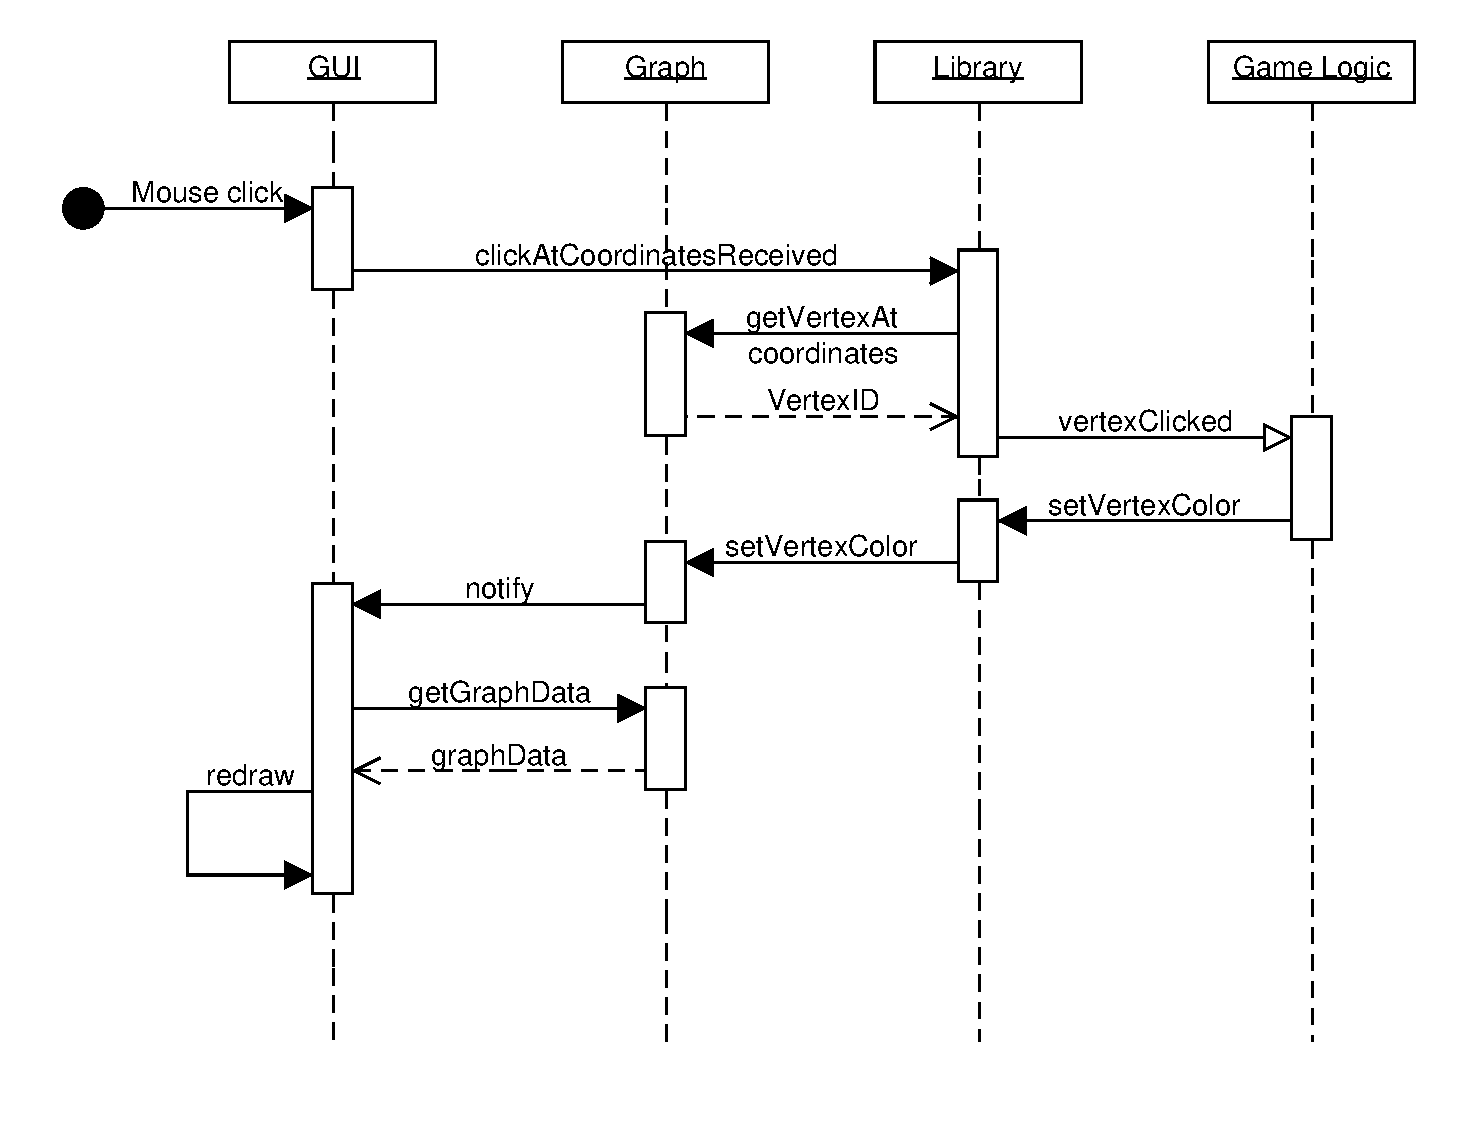
\includegraphics[width=1\textwidth]{sequence.pdf}
	\caption{Example showing the communication between the software components, when a user clicks a vertex to change its color.}
	\label{img:SEQ}
\end{figure}
